\documentclass[a4paper,10pt]{article}
\usepackage[lmargin=2.0cm, rmargin=1.0cm,tmargin=3.5cm,bmargin=1.5cm]{geometry}
\usepackage{color,graphics}
\usepackage[export]{adjustbox}
\usepackage{lipsum}
\usepackage{comment}
\usepackage{graphicx}
\usepackage{grffile}
\usepackage{hyperref}
\usepackage{listings}
\usepackage[scaled=0.75]{helvet}

\usepackage{listings}
\usepackage{color}

\definecolor{dkgreen}{rgb}{0,0.6,0}
\definecolor{gray}{rgb}{0.5,0.5,0.5}
\definecolor{mauve}{rgb}{0.58,0,0.82}

\lstset{frame=tb,
	language=Java,
	aboveskip=3mm,
	belowskip=3mm,
	showstringspaces=false,
	columns=flexible,
	basicstyle={\small\ttfamily},
	numbers=none,
	numberstyle=\tiny\color{gray},
	keywordstyle=\color{blue},
	commentstyle=\color{dkgreen},
	stringstyle=\color{mauve},
	breaklines=true,
	breakatwhitespace=true,
	tabsize=3
}

\begin{document}
\setcounter{secnumdepth}{-1} 

\begin{center}
\textbf{\LARGE Running MapReduce Programs On Single Node Hadoop Cluster - Word Count/Word Frequency}
\end{center}

\raggedright Expt No: 3 \hfill \raggedleft March  06, 2019 \\ 

\raggedright Author: Subalakshmi Shanthosi S  (186001008) \par 

\noindent\makebox[\linewidth]{\rule{\textwidth}{1pt}} 

\section{Aim}
Implementation of MapReduce in Hadoop single node cluster.

\section{Description}
\begin{itemize}
	\item Apache Hadoop
	\begin{itemize}
		\item Large Scale,Open Source Software Framework.
		\item Supports Three Projects:
		\begin{itemize}
			\item Hadoop Common.
			\item HDFS : Hadoop Distributed File System.
			\item MapReduce.
		\end{itemize}
	\end{itemize}
   \item Hadoop MapReduce
     \begin{itemize}
     	\item Hadoop Programming Model and Software Framework.
     	\item Computational Processing:
     	\begin{itemize}
     		\item Unstructured Data : File system
     		\item Structured Data : Database	
     	\end{itemize}
        \item MapReduce Layer has job and task tracker nodes.
        \item Cluster nodes: 
        \begin{itemize}
        	\item Single JobTracker per master.
        	\item Single TaskTracker per slave.
        \end{itemize}
        \item Fundamental Steps:
        \begin{itemize}
        	\item Map Step:
        	\begin{itemize}
        		\item Master node slices problem input into several subproblems input.
        		\item Distributes data slices to worker nodes.
        		\item Worker nodes processes and hands over the control to master.
        	\end{itemize}
           \item Reduce Step: 
           \begin{itemize}
           	\item Master node takes the answers to the sub problems and combines them in a predefined way to get the output/answer to original problem. 
           \end{itemize}
           \end{itemize}
\end{itemize}
\end{itemize}

\section{Software's Used}
\begin{itemize}
  \item Ubuntu  16.04 LTS
  \item Hadoop 1.0.3
\end{itemize}
\pagebreak

\section{Hadoop MapReduce Architecture}
\begin{itemize}
	\item MapReduce Architecture:
	\begin{figure}[h]
		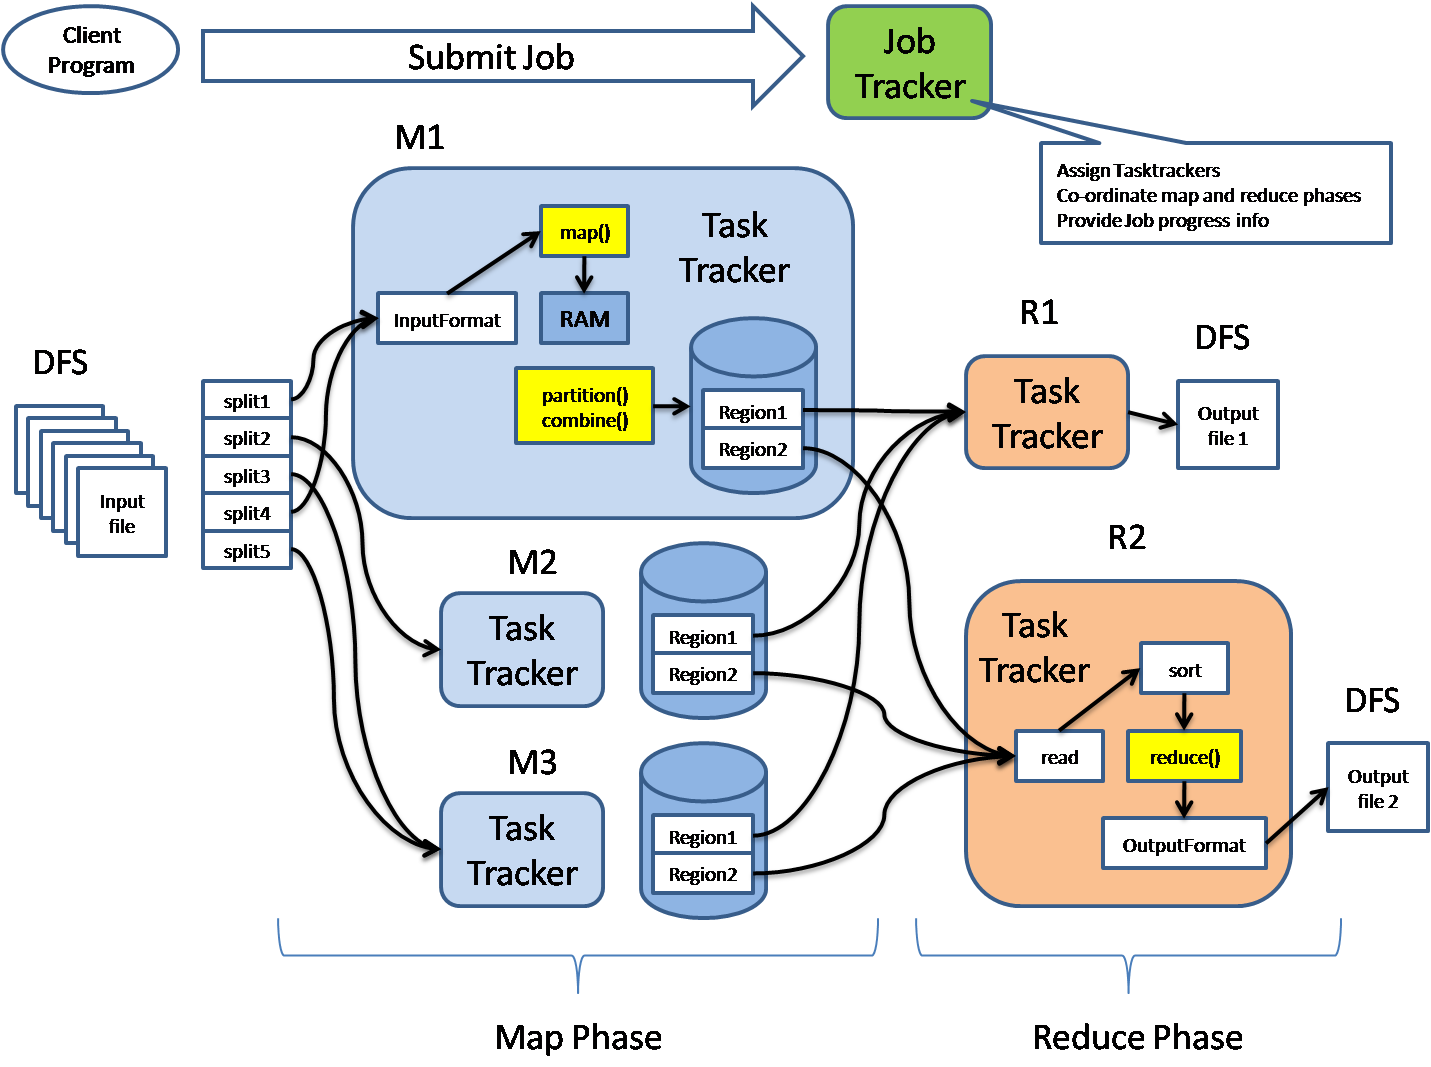
\includegraphics[scale=0.45,center]{exptTwoScreenShot/MapRedArch.png}
		\caption{Hadoop MapReduce Architecture Diagram.}
		\label{fig:0}
	\end{figure}
\end{itemize}

\section{Procedure}

\begin{enumerate}
	\item Launch Ubuntu 16.04 LTS in virtual environment.
	\item Login to the OS with sudo permission and install the following packages using apt-get command
	\begin{itemize}
		\item openssh-server
		\item openssh-client
		\item java jdk 8
		\item javac compiler
        \item hadoop 1.0.3
	\end{itemize}
\pagebreak
  \item Install and configure appropriate environment variables for Hadoop 1.0.3.
  \item Start Hadoop DFS by invoking script start-all.sh in bin directory.
  \item Examine the running Hadoop Job Process using jps command.
  \item Download and place the input files in appropriate directory.
  \item Copy the input Files from Local File System to HDFS using command attribute CopyFromLocal of dfs command.
  \item Run the MapReduce Job.
  \item Retrieve the Job Result from HDFS.
  \item View stats from Web Interface for the following information listed below.
  \begin{itemize}
  	\item JobTracker Web Interface - \url{http://localhost:50030/}
  	\item TaskTracker Web Interface - \url{http://localhost:50060/}
  	\item NameNode Web Interface - \url{http://localhost:50070/} 	
  \end{itemize}
  
\end{enumerate}
\section{Code}
\begin{lstlisting}
// WordCount.java
package org.myorg;
import java.io.IOException;
import java.util.*;
import org.apache.hadoop.fs.Path;
import org.apache.hadoop.conf.*;
import org.apache.hadoop.io.*;
import org.apache.hadoop.mapred.*;
import org.apache.hadoop.util.*;
public class WordCount {

public static void main(String[] args) throws Exception {
	JobConf conf = new JobConf(WordCount.class);
	conf.setJobName("wordcount");
	conf.setOutputKeyClass(Text.class);
	conf.setOutputValueClass(IntWritable.class);
	conf.setMapperClass(Map.class);
	conf.setReducerClass(Reduce.class);
	conf.setInputFormat(TextInputFormat.class);
	conf.setOutputFormat(TextOutputFormat.class);
	FileInputFormat.setInputPaths(conf, new Path(args[0]));
	FileOutputFormat.setOutputPath(conf, new Path(args[1]));
	JobClient.runJob(conf);
}

}
\end{lstlisting}

\begin{lstlisting}
\\Map.java
public static class Map extends MapReduceBase ... {
	private final static IntWritable one = new IntWritable(1);
	private Text word = new Text();
	public void map(LongWritable key, Text value,
	OutputCollector<Text, IntWritable> output, ...) ... {
	String line = value.toString();
	StringTokenizer tokenizer = new StringTokenizer(line);
	while (tokenizer.hasMoreTokens()) {
		word.set(tokenizer.nextToken());
		output.collect(word, one);
		} } }
\end{lstlisting}
\begin{lstlisting}
\\Reduce.java
public static class Reduce extends MapReduceBase ... {
	public void reduce(Text key, Iterator<IntWritable> values,
	OutputCollector<Text, IntWritable> output, ...) ... {
	int sum = 0;
	while (values.hasNext()) {
		sum += values.next().get();
		}
	output.collect(key, new IntWritable(sum));
		}
	}
}
\end{lstlisting}
\section{Output}
\begin{figure}[h]
	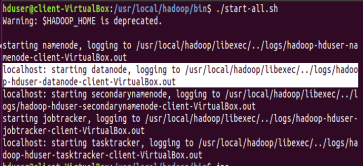
\includegraphics[scale=0.55,center]{exptTwoScreenShot/fig1.png}
	\caption{Starting Hadoop DFS.}
	\label{fig:1}
	
\end{figure}
\begin{figure}[h]
	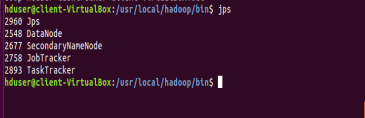
\includegraphics[scale=0.54,center]{exptTwoScreenShot/fig2.png}
	\caption{Examining Running Hadoop Process.}
	\label{fig:2}
\end{figure}

\begin{figure}[h]
	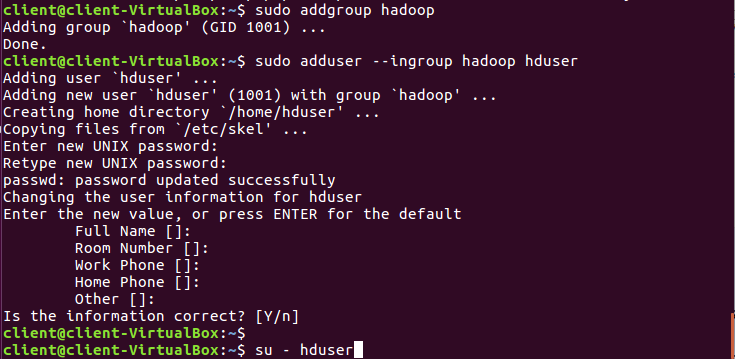
\includegraphics[scale=0.44,center]{exptTwoScreenShot/fig3.png}
	\caption{Placing the inputFiles in appropriate location.}
	\label{fig:3}
\end{figure}
\newpage

\begin{figure}[h]
	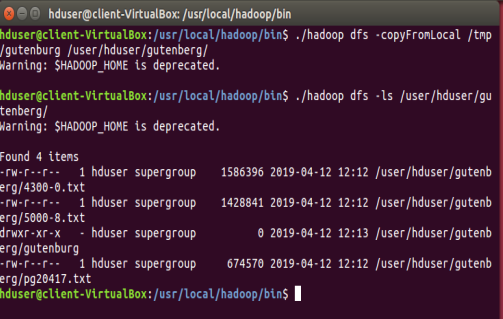
\includegraphics[scale=0.34,center]{exptTwoScreenShot/fig4.png}
	\caption{Copy Files from Local to HDFS.}
	\label{fig:4}
\end{figure}

\begin{figure}[h]
	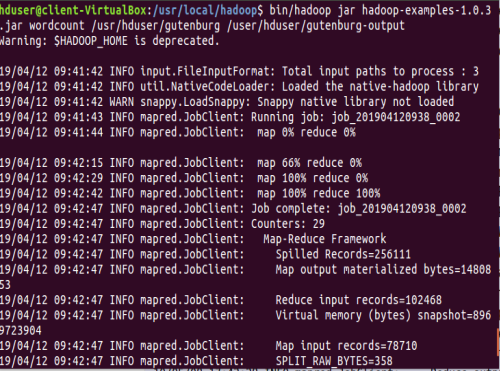
\includegraphics[scale=0.30,center]{exptTwoScreenShot/fig5.png}
	\caption{Run MapReduce Task for Input Files.}
	\label{fig:5}
\end{figure}
\begin{figure}[h]
	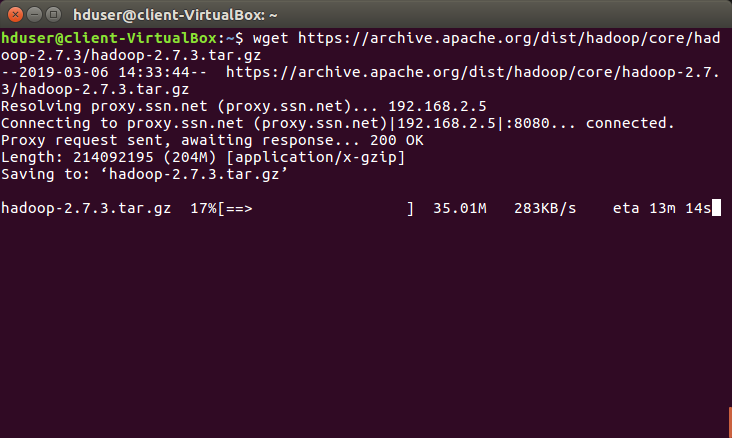
\includegraphics[scale=0.50,center]{exptTwoScreenShot/fig6.png}
	\caption{Retrieve Hadoop MapReduce Output from appropriate folder.}
	\label{fig:6}
\end{figure}

	\begin{figure}[h]
		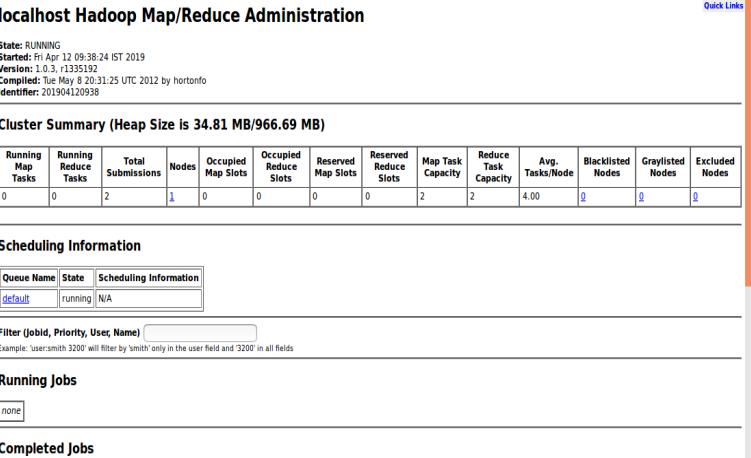
\includegraphics[scale=0.30,center]{exptTwoScreenShot/fig7.png}
		\caption{JobTracker of HDFS Web Interface.}
		\label{fig:7}
	\end{figure}
	
	\begin{figure}[h]
		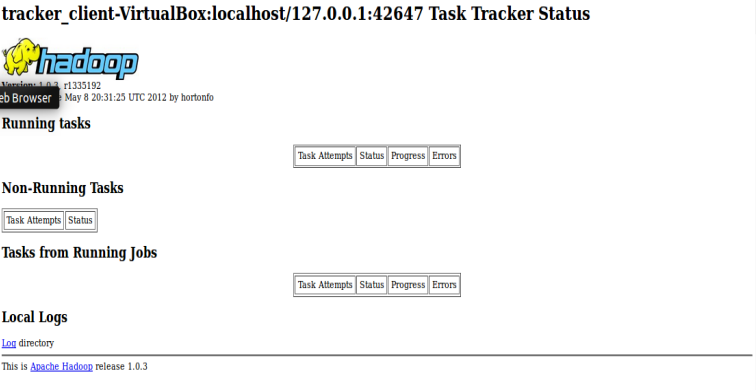
\includegraphics[scale=0.30,center]{exptTwoScreenShot/fig8.png}
		\caption{Task Tracker of HDFS Web Interface.}
		\label{fig:8}
	\end{figure}

\pagebreak

	\begin{figure}[h]
		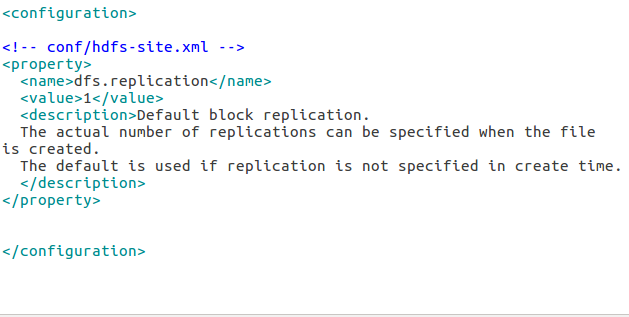
\includegraphics[scale=0.30,center]{exptTwoScreenShot/fig9.png}
		\caption{Web Interface of HDFS Namenode.}
		\label{fig:10}
	\end{figure}
  
\section{Result}
Thus the hadoop MapReduce program for finding word cound and frequency was successly executed and its results in Web Interface for a better understanding.

\end{document}
